\section{Data, cakupan, dan klasifikasi barang}\label{sec:data}
\subsection{Asal perdagangan dan arti kode mitra}
Perdagangan berasal dari 22 workbook Trade Map pengguna: ekspor dan impor Indonesia terhadap sepuluh mitra serta seluruh negara. Semua file menuliskan Indonesia, kode pelapor 360, pada sisi eksportir untuk file ekspor dan sisi importir untuk file impor. Kode 000 atau \texttt{World} pada file agregat adalah mitra seluruh dunia. Audit tambahan mencocokkan 5.456 nilai TOTAL bulanan dengan panel intermediate. Kecocokan ini memastikan asal dan transformasi internal, tetapi belum menggantikan validasi statistik independen terhadap sumber nasional.

Kolom \texttt{ISO3} pada panel menunjukkan mitra, bukan negara pelapor. Baris \texttt{WLD} adalah perdagangan Indonesia dengan seluruh mitra, sedangkan \texttt{CHN} adalah perdagangan Indonesia dengan Tiongkok. Dalam model barang kunci diperluas dengan kelompok. Tabel lampiran memakai kode yang sama untuk menghemat ruang.

\subsection{Frekuensi, satuan, dan agregasi}
Workbook memuat nilai bulanan Januari 2006--Agustus 2026 dalam USD ribu. Nilai dijumlahkan untuk membentuk kuartal. Kuartal hanya lengkap ketika ketiga bulan tersedia; Juli--Agustus 2026 belum membentuk kuartal ketiga lengkap. Nol eksplisit dipertahankan. Blank tidak diubah menjadi nol, meskipun audit tidak menemukan kekosongan numerik pada sel nilai perdagangan yang diimpor.

Baris TOTAL dipakai untuk agregat dan bilateral. Kelompok dihitung dari kode HS-6 yang memenuhi definisinya. Jumlah produk dibandingkan dengan TOTAL menurut batas pembulatan per baris. Selisih relatif maksimum audit sekitar 0,0483\%, dan semuanya berada dalam batas pembulatan yang digunakan. Selisih kecil akibat pembulatan tidak dipaksa menjadi nol atau langsung dianggap produk yang hilang.

Konversi USD ribu ke USD miliar dilakukan dengan membagi satu juta. Pada 2025 ekspor Indonesia mencapai USD \WorldExports{} miliar, impor USD \WorldImports{} miliar, dan neraca USD \WorldNet{} miliar. Tahun 2025 digunakan karena lengkap. Statistik sampel estimasi mengikuti tanggal regresi, sehingga berbeda dari statistik seluruh raw data.

\begin{figure}[!htbp]\centering
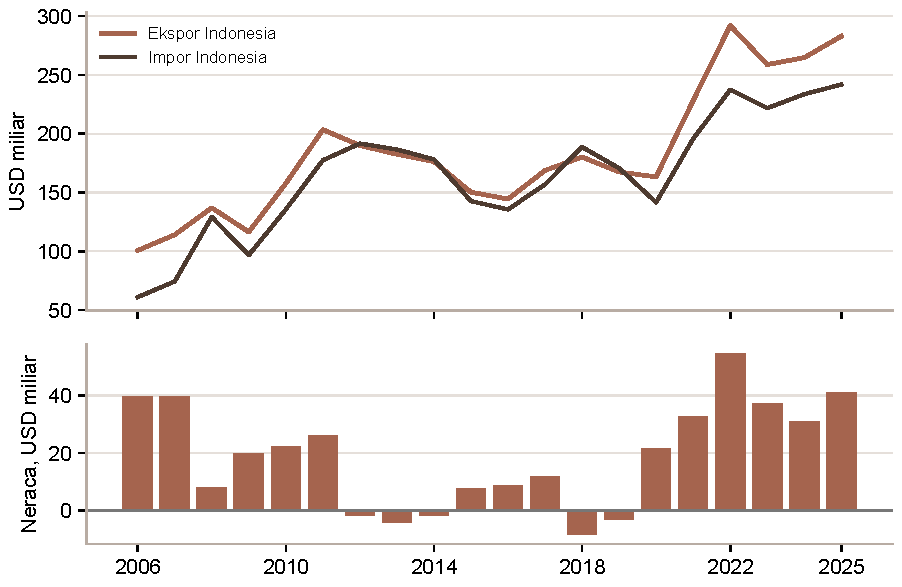
\includegraphics[width=\linewidth]{assets/indonesia_annual.pdf}
\caption{Ekspor, impor dan neraca perdagangan barang Indonesia terhadap seluruh negara. Nilai tahunan hanya menggunakan empat kuartal lengkap. Sumber: workbook Trade Map dan panel kuartalan proyek.}\label{fig:annual}
\end{figure}

\subsection{Dua dimensi klasifikasi yang bertumpang tindih}
Klasifikasi komoditas memakai kelompok A11 UNCTAD melalui korespondensi HS--SITC \cite{unctad,unsdcorr}. Komoditas total mencakup pangan, minuman, tembakau, minyak, bahan mentah pertanian, bahan bakar, serta bijih, mineral dan komoditas logam tertentu. Pertanian/pangan dan energi/tambang digunakan sebagai rinciannya. Manufaktur nonkomoditas mengikuti kategori pelengkap pada aturan tersebut, bukan identifikasi industri setiap perusahaan.

Konsumsi, modal, dan bahan baku/penolong memakai dimensi penggunaan SNA dalam BEC Rev.5 \cite{bec}. Penggunaan ini berbeda dari sifat komoditas. Produk pertanian dapat menjadi konsumsi akhir atau input antara; produk manufaktur dapat menjadi input maupun modal. Tujuh kelompok karena itu tidak merupakan partisi eksklusif. Menjumlahkan semuanya menghitung sebagian arus lebih dari sekali.

\begin{table}[!htbp]\centering\small
\caption{Kode dan definisi tujuh kelompok barang}
\begin{tabular}{p{.07\linewidth}p{.29\linewidth}p{.53\linewidth}}
\toprule Kode & Kelompok & Dasar pembentukan\\\midrule
G1 & Manufaktur nonkomoditas & Nonkomoditas UNCTAD A11 melalui SITC.\\
G2 & Barang konsumsi & BEC Rev.5, penggunaan konsumsi akhir.\\
G3 & Pertanian dan pangan & Komoditas pangan dan bahan mentah pertanian.\\
G4 & Bahan baku/penolong & BEC Rev.5, penggunaan konsumsi antara.\\
G5 & Barang modal & BEC Rev.5, pembentukan modal tetap.\\
G6 & Komoditas total & Seluruh komoditas A11 yang dapat dipetakan.\\
G7 & Energi dan tambang & Bahan bakar, bijih/mineral dan komoditas logam terkait.\\
\bottomrule\end{tabular}\label{tab:groups}
\end{table}

Workbook tidak menyatakan revisi HS untuk setiap sel. Daftar memuat kode dari beberapa revisi, sehingga kelas ditetapkan dengan konsensus konservatif per kode dari korespondensi resmi. Bila kemungkinan kelas berbeda, nilai ditandai campuran atau belum terpetakan. Nilainya tetap dalam TOTAL dan tidak dipaksakan ke kelompok tertentu. Cakupan dihitung juga per tahun, agar perubahan kode dan komposisi terlihat.

Konsensus per kode lebih rinci daripada klasifikasi HS-4, tetapi belum menjadi harmonisasi produk lintas waktu yang sempurna. Komposisi di dalam kelompok dapat berubah; hasil kelompok tidak berarti setiap kode atau perusahaan mempunyai respons sama. Kategori bahan baku/penolong menunjukkan penggunaan barang, bukan kandungan input impor eksportir.

\subsection{Kontrol makro dan keterbatasan pengukuran}
Aktivitas ekonomi menggunakan indeks level PDB riil yang ditransformasi log. Indeks pada basis rata-rata 2015 tidak boleh dijumlahkan sebagai nilai uang lintas negara. Pada bilateral digunakan GDP mitra. Pada agregat digunakan indeks sepuluh mitra dengan bobot ekspor tetap 2006--2008 dari data baru. Proksi itu merepresentasikan sebagian permintaan eksternal, tidak setara dengan GDP seluruh dunia.

Kurs agregat memakai REER BIS. Kurs bilateral dibangun dari kurs nominal dan harga, kemudian orientasinya diseragamkan agar kenaikan berarti apresiasi. Guncangan penelitian adalah perubahan kurs riil; besarnya tidak otomatis sama dengan perubahan nominal rupiah terhadap dolar. Indeks BCOM dari workbook pengguna digunakan sebagai kontrol tambahan pada sensitivitas.

India memakai CPI mulai 2013, dengan WPI sebagai pembanding terpisah. CPI Australia bulanan memuat interpolasi penyedia. Kekosongan CPI AS Oktober 2025 dan FX Vietnam Agustus 2025 dipertahankan. Beberapa GDP historis serta konsep kurs antarkompiler mempunyai catatan audit. Jejak sumber tersedia, tetapi keseragaman konsep dan vintage belum sepenuhnya terselesaikan.

\subsection{Penentuan sampel dan statistik deskriptif}
Setiap kasus memilih jendela lengkap terpanjang pada kalender kuartalan. Kuartal kosong tidak dihapus lalu dianggap berurutan. Ini menjaga arti lag, tetapi menghasilkan rentang berbeda. Baseline agregat dimulai pada data 2010Q1 demi pembandingan dengan run sebelumnya; sesudah holdback empat lag, estimasi mencakup 2011Q1--2026Q1. Perluasan 2006+ disajikan sebagai sensitivitas.

\begin{table}[!htbp]\centering
\caption{Statistik sampel estimasi agregat Indonesia, 2011Q1--2026Q1}
{\small\setlength{\tabcolsep}{3pt}\renewcommand{\arraystretch}{1.15}
\begin{tabular}{p{0.32\linewidth}p{0.045\linewidth}p{0.12\linewidth}p{0.12\linewidth}p{0.12\linewidth}p{0.12\linewidth}}
\toprule
\textbf{Variabel} & \textbf{N} & \textbf{Rerata} & \textbf{SD} & \textbf{Min.} & \textbf{Maks.}\\
\midrule
Ekspor, USD miliar & 61 & 51,15 & 12,46 & 33,60 & 78,20\\
Impor, USD miliar & 61 & 46,92 & 9,06 & 31,73 & 65,54\\
Neraca, USD miliar & 61 & 4,24 & 5,08 & -4,80 & 15,61\\
PDB riil Indonesia, indeks & 61 & 114,85 & 21,27 & 79,40 & 156,49\\
Aktivitas luar negeri, indeks & 61 & 109,43 & 13,98 & 86,16 & 135,66\\
REER, indeks & 61 & 100,99 & 4,32 & 92,89 & 111,01\\
\bottomrule
\end{tabular}
}\label{tab:desc}
\end{table}

Ekspor dan impor dalam Tabel~\ref{tab:desc} adalah nilai per kuartal. Neraca yang reratanya positif masih mempunyai kuartal defisit. Level surplus nasional karena itu tidak menjelaskan pengaruh kurs dengan sendirinya. Perdagangan belum disesuaikan musiman, sedangkan sebagian GDP memakai seri penyedia yang telah disesuaikan. Musiman masih perlu diperiksa.
